\chapter{Multi Layer Perception}

The multi layer perception is the most known and most frequently used type of neural network. It consists of at least three layers. The difference between Multi and Single layer perception is that, the first one can learn non-linear functions, whereas the second one is only suitable for solving linear problems. 

Multilayer perceptrons are often applied to supervised learning problems: they are being trained on a set of input-output pairs and learn to model the dependencies between the given inputs and outputs. Training, so-called backpropagation, involves adjusting the parameters of the model in order to minimize the error. MLP performs well with relatively low dimensional inputs. 


\section{Implementation and test result}
Due to the big amount of parameters its rather a poor solution for working with the images as its inputs. To proceed with MLP algorithm we need relatively low dimensional data. The idea to implement Face Recognition system using MLP is to connect Multi Layer Perception model with Principal Component Analysis algorithm. 

The first step in this approach is to perform PCA on every image in a training data set. PCA produces a weight vector, (4.13) for an image, hence we can represent each image in a low dimensional space. The dimension depends on the number of eigenvectors chosen for Principal Component Analysis algorithm. 

\begin{equation}
X =
\left[
\begin{matrix}
w_{11} & w_{21} & \cdots & \cdots & w_{m1}\\
w_{12} & w_{22} & \cdots & \cdots & w_{m2}\\
w_{13} & w_{23} & \cdots & \cdots & w_{m3}\\
w_{14} & w_{24} & \cdots & \cdots & w_{m4}\\
\cdots & \cdots & \cdots & \cdots & \cdots\\
\cdots & \cdots & \cdots & \cdots & \cdots\\
w_{1k} & w_{2k} & \cdots & \cdots & w_{mk}
\end{matrix}
\right]
\end{equation}

where $k$ is a number of eigenvectors and $m$ is amount of data in a training data set.

Since the MLP is a supervised algorithm, to train the model the data labels are required. Each label was represented as a k-dimensional vector.

\begin{equation}
Y =
\left[
\begin{matrix}
0 & 1 & \cdots & \cdots & 0\\
0 & 0 & \cdots & \cdots & 0\\
0 & 0 & \cdots & \cdots & 1\\
1 & 0 & \cdots & \cdots & 0\\
\cdots & \cdots & \cdots & \cdots & \cdots\\
\cdots & \cdots & \cdots & \cdots & \cdots\\
0 & 0 & \cdots & \cdots & 0
\end{matrix}
\right]
\end{equation}

The goal is to train the model in a way that given the matrix $X$ MLP will produce close approximation of matrix $Y$. 

For training the model backpropagation algorithm was used. 
\\
\begin{python}
def back_prop(epochs, X, Y, Wh, Wp, activation, l_rate):
    for i in range(epochs):
        H = activation(np.dot(X, Wh))  
        Z = activation(np.dot(H, Wp)) 
        E = error(Y, P)
        dP = E * activation(Z, deriv=True) 
        dH = dP.dot(Wp.T) * activation(H, deriv = True)  
        Wz += l_rate * H.T.dot(dP)  
        Wh += l_rate * X.T.dot(dH)  
        if i % 10000 == 0:
            per = check_performance(Z)
            if per > 0.98:
                break
\end{python}


The neural network performance varies depending on the change of various parameters such as:

\begin{itemize}
\itemsep0em 
\item amount of input data
\item amount of neurons in hidden layers
\item initial weights
\item activation function
\item learning parameter
\end{itemize}

The tests were performed on two different databases: 
\begin{itemize}
\itemsep0em 
\item Chicago Face Database - pictures captured in controlled environment
\item Labeled Faces in Wild database - pictures captured in uncontrolled environment, with various lightning conditions, pose, facial expression etc. 
\end{itemize}


\section{Tests on pictures captured in controlled environment}

The database was divided into training and testing samples. The training was performed using 3 pictures of the individual, one pictures was used to test the trained model. 

\begin{figure}[H]
\centering
\begin{subfigure}[b]{.2\linewidth}
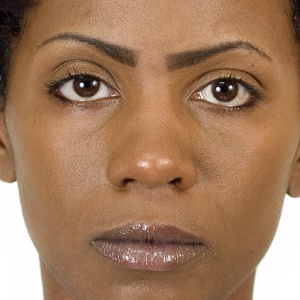
\includegraphics[width=\linewidth]{img/CFD1.jpg}
\end{subfigure}
\centering
\begin{subfigure}[b]{.2\linewidth}
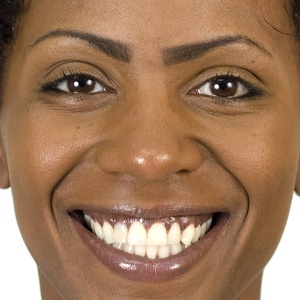
\includegraphics[width=\linewidth]{img/CFD2.jpg}
\end{subfigure}
\centering
\begin{subfigure}[b]{.2\linewidth}
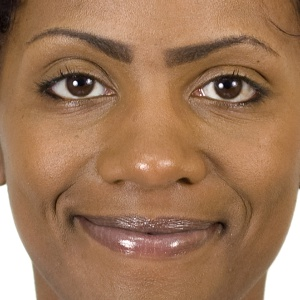
\includegraphics[width=\linewidth]{img/CFD3.jpg}
\end{subfigure}
\caption{Examples of one person pictures in the training dataset}
\end{figure}


\begin{figure}[H]
\centering
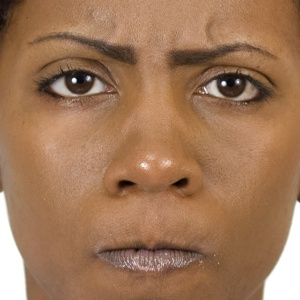
\includegraphics[scale=0.3]{img/CFD4.jpg}
\caption{Testing image}
\end{figure} 


The tests were performed using MLP topology presented on figure 7.1 (???).

\begin{figure}[!h]
\centering
\begin{tikzpicture}[
           > = Stealth, semithick,
plain/.style = {draw=none, fill=none, yshift=11mm,
                text width=7ex,  align=center},% for text in images, 
   ec/.style = {draw=none},% for emty cells
  net/.style = {% for matrix style
    matrix of nodes,
    nodes={circle, draw, semithick, minimum size=12mm, inner sep=0mm},% circles in image
    nodes in empty cells,% for not used cells in matrix
  column sep = 16mm, % distance between columns in matrix 
     row sep = -3mm  % distance between rows in matrix
            },
]
\matrix[net] (m)% m is matrix name, it is used for names of cell: firs has name m-1-1
                % in empty space between ampersands will show circles: 
                % i.e.: nodes of the neural network
{
|[plain]| $Input$ & |[plain]| $Hidden$ & |[plain]| $Output$ \\
|[ec]|                &                         & |[ec]|                  \\
                      & |[ec]|                  & |[ec]|                  \\
|[ec]|                &                         &                         \\
                      & |[ec]|                  & |[ec]|                  \\
|[ec]|                &                         &                         \\
                      & |[ec]|                  & |[ec]|                  \\
|[ec]|                &                         & |[ec]|                  \\
};
\% inputs
\foreach \in [count=\ir from 1] in {3,5,7}
\draw[<-] (m-\in-1.west) -- node[above]{}+(-12mm,0);
% connections between nodes in the first and second layer
\foreach \j in {3,5,7}
{
\foreach \k in {2,4,6,8} \draw[->] (m-\j-1) -- (m-\k-2);
}
% connections between nodes in the second and third layer
\foreach \j in {2,4,6,8}
{
\foreach \k in {4,6} \draw[->] (m-\j-2) -- (m-\k-3);
}
% output
\draw[->] (m-4-3.east) -- node[above] {} +(12mm,0);
\draw[->] (m-6-3.east) -- node[above] {} +(12mm,0);
    \end{tikzpicture}
\caption{Neural Network with one hidden layer}
\end{figure}


\subsection{20 individuals}

The first step is to set a number of eigenvectors that the image will be represented with. We do it using previously implemented PCA algorithm. 

\begin{figure}[H]
\centering
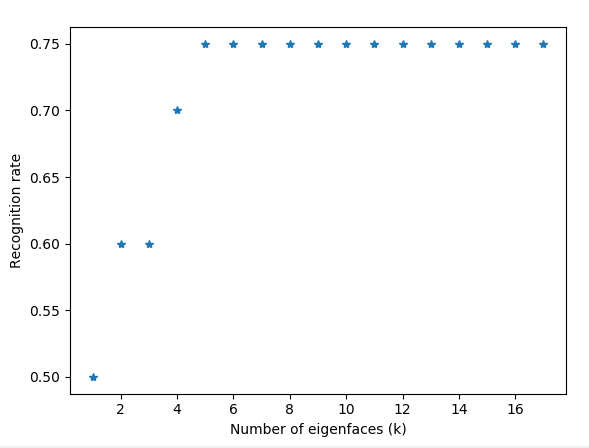
\includegraphics[scale=0.7]{img/tests/20ppl/PCA_on_20ppl_vs_k.png}
\caption{Recognition rate with varying number of eigenvectors for 20 individuals}
\end{figure} 

From this results, we can conclude that $k = 6$ is the sufficient amount of eigenvectors to properly represent each sample image. 

Test was performed on a data set with 20 individuals.
The PCA-MLP algorithm was ran with following parameters:

\begin{itemize}
\itemsep0em 
\item number of hidden layers = 1
\item number of neurons in hidden layers = 10
\item initial weights chosen randomly in a range [0:1]
\item sigmoid activation function
\item learning parameter = 1
\item number of eigenvectors $k = 6$
\end{itemize}

In order to examine accuracy of PCA-MLP algorithm we check if the index of obtained outputs' maximum value is equal to the index of maximum value of desired output. The accuracy is a value representing percentage of pictures that fulfills this requirement.

As the first step the influence of a learning rate parameter was examined.\\
\textbf{Learning rate = 1}\\
\begin{figure}[H]
\centering
\begin{subfigure}[b]{.45\linewidth}
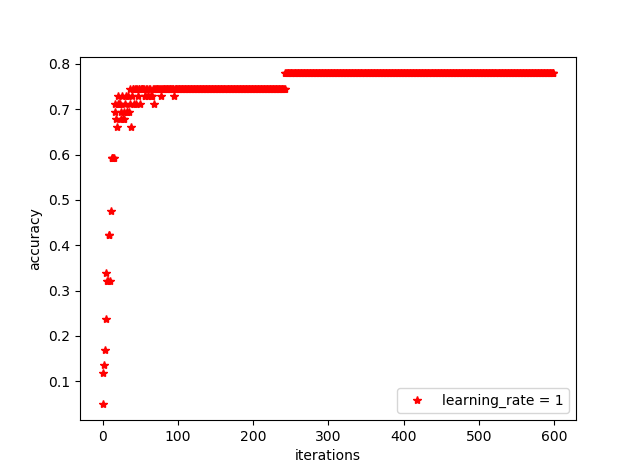
\includegraphics[width=\linewidth]{img/tests/20ppl/learnig_rate1_v1.png}
\end{subfigure}

\begin{subfigure}[b]{.45\linewidth}
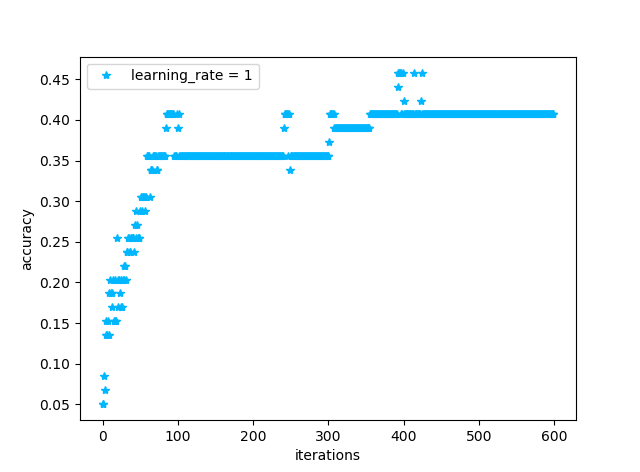
\includegraphics[width=\linewidth]{img/tests/20ppl/learnig_rate1_v2.png}
\end{subfigure}
\begin{subfigure}[b]{.45\linewidth}
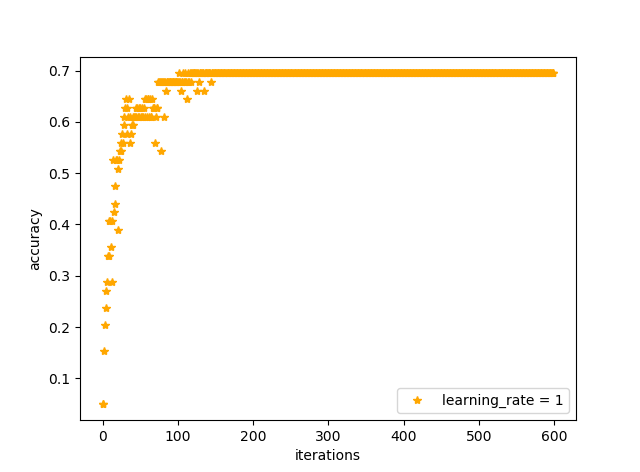
\includegraphics[width=\linewidth]{img/tests/20ppl/learnig_rate1_v3.png}
\end{subfigure}
\caption{Learning rate = 1, initial weights chosen randomly}
\label{fig:animals}
\end{figure}

The neural network with learning rate = 1 is very unstable and strongly depends on initial weights. 

The tests were performed for different learning rate values:

\begin{figure}[H]
\centering
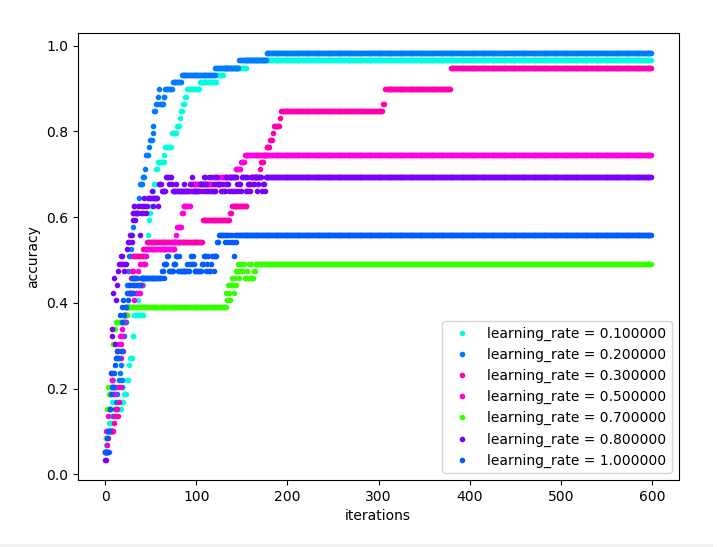
\includegraphics[scale=0.7]{img/tests/20ppl/learning_rates.png}
\caption{Algorithm accuracy with different learning rates}
\end{figure}

The learning rate is one of the most important hyper-parameters to tune for training neural networks. If the learning rate is low, then training is more reliable, but optimization will take more time because the weights changes are tiny.

For each experiment approximately 400 iterations were enough to sufficiently train the network.
 
To compare the accuracy of PCA algorithm itself with connection of PCA and MLP algorithms, the PCA results should be examined. The highest obtained recognition rate ( figure 7.4)  is 0.75.

The testing phase was made using the model that was train with following parameters:

\begin{itemize}
\itemsep0em
\item number of hidden layers = 1
\item number of neurons in hidden layers = 10
\item initial weights chosen randomly in a range [0:1]
\item sigmoid activation function
\item learning parameter = 0.2
\item number of eigenvectors $k = 6$
\end{itemize}


Obtained results are good. 18 out of 20 people were recognized correctly - the recognition rate reached 90\%, which is 15 percentage points better than result of PCA algorithm.


\subsection{40 individuals}

The choice of a number of eigenvectors representing the images in a small database is straightforward as presented in section (???). 

Following the same procedure as in section (???) we can derive the optimal (for PCA algorithm) $k$ value. 

\begin{figure}[H]
\centering
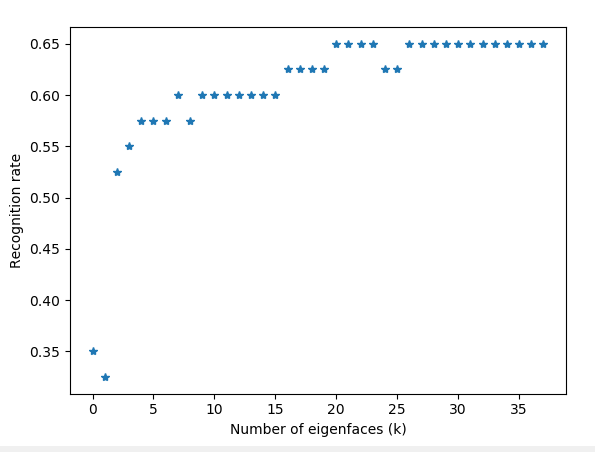
\includegraphics[scale=0.5]{img/tests/40ppl/PCA_40.png}
\caption{Recognition rate with varying number of eigenvectors for 40 individuals}
\end{figure} 

When dealing with a bigger database, we have to find a balance between a sufficient amount of eigenfaces to represent an image and an amount of data that can be applied as the input of multilayer perception network, so that we'll obtain acceptable training result in a reasonable time. The bigger input dimension, the harder it is to train the network. 

In this case input dimension = 27 is still low enough to be processed with MLP network, hence parameter $k$ was set to 27.

Test was performed with following parameters:

\begin{itemize}
\itemsep0em
\item dimension of input data = 27
\item number of hidden layers = 1
\item number of neurons in hidden layers = 27
\item initial weights chosen randomly in a range [0:1]
\item sigmoid activation function
\item learning rate = 0.2
\end{itemize}

The result of training algorithm. 

\begin{figure}[H]
\centering
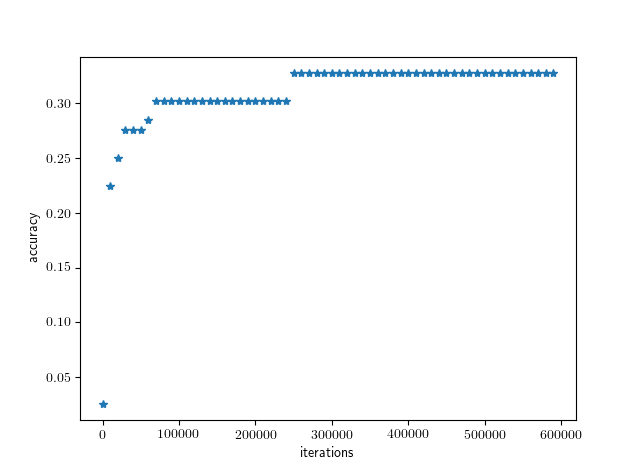
\includegraphics[scale=0.5]{img/tests/40ppl/k=27,h=27,60000epoch/res.png}
\caption{number of eigenvectors = 27, number of hidden neurons = 27}
\end{figure} 

The execution of the algorithm took 4 min 54 sek. The results are not satisfying.  

The next interesting parameter in terms of neural network performance is a number of neurons in a hidden layer. This topic is still an active area of research, and the major answers are driven by tests and experience. In the previous experiment, amount of hidden neurons was equal to the amount of input neurons and it does not seem to be a good solution. The recognition rate in the network trained as such reached 22,5\%, which is rather poor. The next step is to check if increasing or decreasing the amount of neurons in a hidden layer will help to improve the network performance. 

Using too few neurons in the hidden layers will result in underfitting. Underfitting occurs when there are too few neurons in the hidden layer to adequately detect the signals in a complicated data set.

On the other hand too many neurons in the hidden layer can result in several problems.
First of all overfitting - occurs when the neural network has so much information processing capacity that the limited amount of information contained in the training set is not enough to train all of the neurons in the hidden layers. Second of all, there is another problem that can be encountered even if the training data is sufficient. A large number of neurons in the hidden layer can increase the time it takes to train the network. The proper compromise must be reached between too many and too few neurons in the hidden layer.

There are several rule-of-thumb methods for determining an sufficient number of neurons in the hidden layers, such as the following:

\begin{itemize}
\itemsep0em 
\item The number of hidden neurons should be between the size of the input layer and the size of the output layer.
\item The number of hidden neurons should be 2/3 the size of the input layer, plus the size of the output layer.
\item The number of hidden neurons should be less than twice the size of the input layer.
\end{itemize}

In our case we have 27 input neurons and 40 output neurons. According to the listed rules we have 3 possibilities:

\begin{enumerate}
\itemsep0em 
\item the amount of hidden neurons should be in range between $27$ and $40$. 
\item the amount of hidden neurons should be equal to $0.6 * 27 + 40 \sim 56$
\item the amount of hidden neurons should be less than $\frac{27}{2} = 13.5$
\end{enumerate}

Each of the possibilities was examined. The results not only differ in the accuracy of the algorithm but also in the execution time. 

\begin{figure}[H]
\centering
\begin{subfigure}[b]{.45\linewidth}
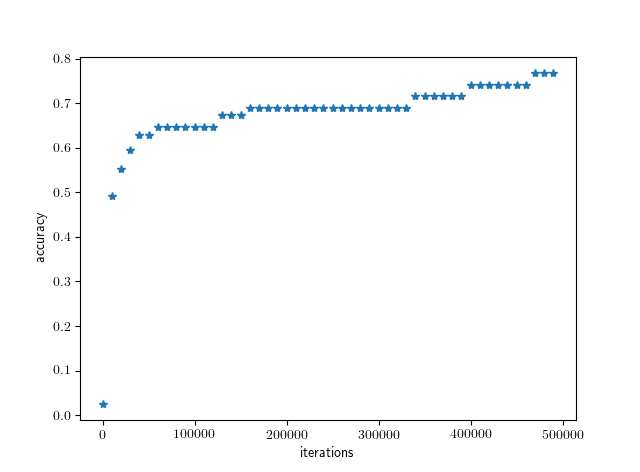
\includegraphics[width=\linewidth]{img/tests/40ppl/k=27,h=10,50000epoch/res.png}
\caption{10 hidden layers}
\end{subfigure}

\begin{subfigure}[b]{.45\linewidth}
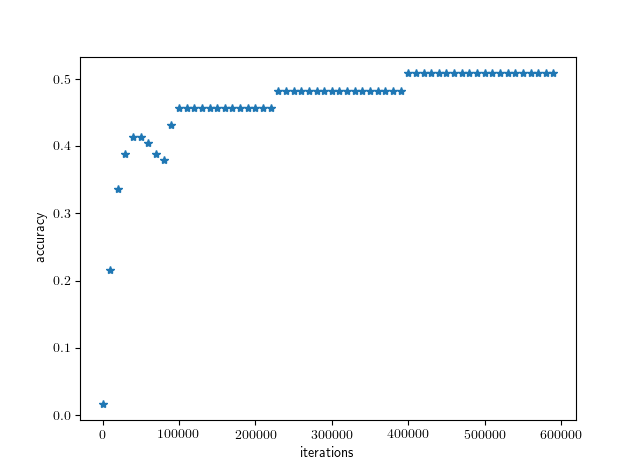
\includegraphics[width=\linewidth]{img/tests/40ppl/k=27,h=33,60000epoch/res.png}
\caption{33 hidden layers}
\end{subfigure}
\begin{subfigure}[b]{.45\linewidth}
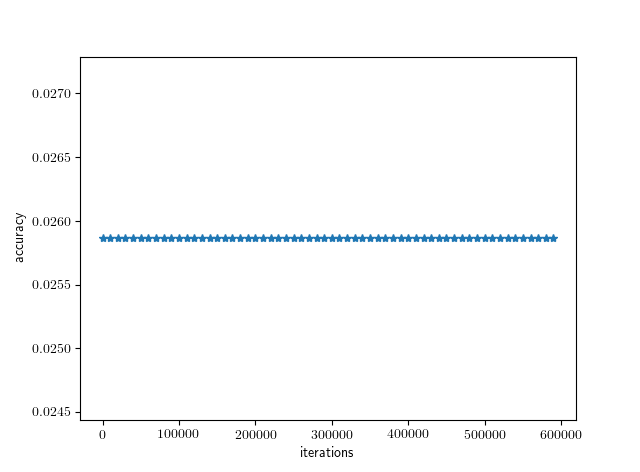
\includegraphics[width=\linewidth]{img/tests/40ppl/k=27,h=56,60000epoch/res.png}
\caption{56 hidden layers}
\end{subfigure}
\caption{Training accuracy for different amount of hidden neurons}
\end{figure}

\begin{center}
    \begin{tabular}{ | l | l | l | p{5cm} |}
    \hline
    Number of hidden neurons &  $10$ & $33$ & $56$ \\ \hline
    Execution time[sek] &  $114$  & $173$ & $216$ \\ \hline
	Recognition Rate & $70\%$ & $43.5\%$ & $2.5\%$ \\ \hline
    Training accuracy & $76.5\%$ & $50\%$ & $2.5\%$\\
    \hline
    \end{tabular}
\end{center}

The best results were achieved with 10 hidden layers. Comparing these results with the result of PCA algorithm on the same data, it seems that the performance of both is very similar. The reason for that might be not sufficient amount of training data. There is a technique that is facing this problem - so-called data augmentation.

It is a widely used method in many machine learning tasks to enlarge the training data set size and avoid overfitting. The goal of this process is to create new samples from the original training data by, for example, flipping, distorting, adding a small amount of noise to, or cropping a patch from an original image.

The first transformation is shifting  the image in four directions - left, right, down, up.


\begin{figure}[H]
\centering
\begin{subfigure}[b]{.3\linewidth}
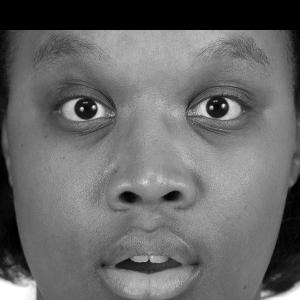
\includegraphics[width=\linewidth]{img/tests/shifts/shifted_image0.jpg}
\end{subfigure}
\centering
\begin{subfigure}[b]{.3\linewidth}
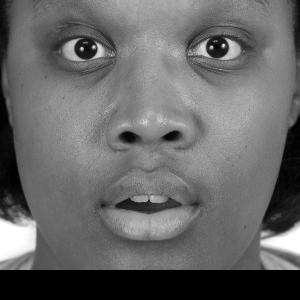
\includegraphics[width=\linewidth]{img/tests/shifts/shifted_image1.jpg}
\end{subfigure}


\begin{subfigure}[b]{.3\linewidth}
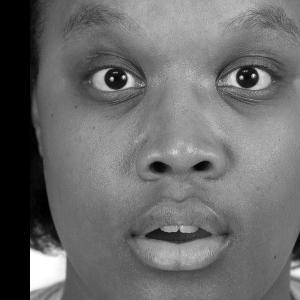
\includegraphics[width=\linewidth]{img/tests/shifts/shifted_image2.jpg}
\end{subfigure}
\begin{subfigure}[b]{.3\linewidth}
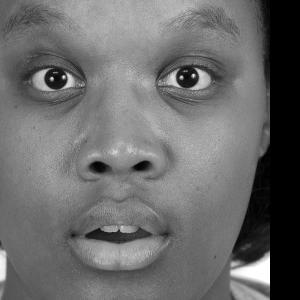
\includegraphics[width=\linewidth]{img/tests/shifts/shifted_image3.jpg}
\end{subfigure}
\caption{Shift transformations}
\end{figure}

Another applied image transformation is flipping the content of the image from left to right.

\begin{figure}[H]
\centering
\begin{subfigure}[b]{.3\linewidth}
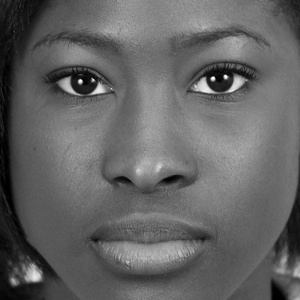
\includegraphics[width=\linewidth]{img/tests/shifts/image.jpg}
\end{subfigure}
\centering
\begin{subfigure}[b]{.3\linewidth}
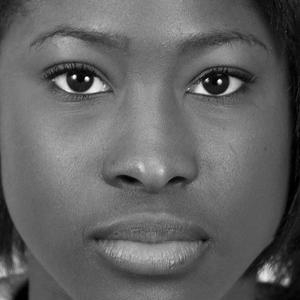
\includegraphics[width=\linewidth]{img/tests/shifts/flipped_image.jpg}
\end{subfigure}
\caption{Flipping transformation}
\end{figure}

Increasing amount of training data makes the training process much longer. It took about 15 min to train the network. In our case the results did not improve, but this is mainly because the training data is not varied in terms of shifting. The face is always in the same position in the picture. 
The recognition rate was 42,5\%, which is much worse, then before enlarging the data set. 
 
The algorithm was tested with Chicago Face Database, where all the individuals were captures in controlled environment. 
The samples of each individual differs only in terms of face expression. It is much more challenging to build a system that is not sensitive for changing the light conditions, the picture quality, face pose and many other factors. 

\section{Tests on pictures captured in uncontrolled environment}

To test the algorithm the Labeled Faces in Wild database was used. The quality of images is much worse then in the previous examples, so the tests result are expected to be worse. 


\begin{figure}[H]
\centering
\begin{subfigure}[b]{.2\linewidth}

\includegraphics[width=\linewidth]{img/tests/lwf/sample1.jpg}
\end{subfigure}
\centering
\begin{subfigure}[b]{.2\linewidth}

\includegraphics[width=\linewidth]{img/tests/lwf/sample2.jpg}
\end{subfigure}
\caption{Exemplary samples from LFW database}
\end{figure}

Test was performed on 20 individuals with 30 pictures each. The training set for each person consists of 27 samples, 3 pictures were used to test the model. 

\subsection{One hidden layer}

The tests were performed in the same topology as presented in figure(??)

As in the previous examples PCA was performed as a first step. The results (figure 7.13) are very poor as expected. 

\begin{figure}[H]
\centering
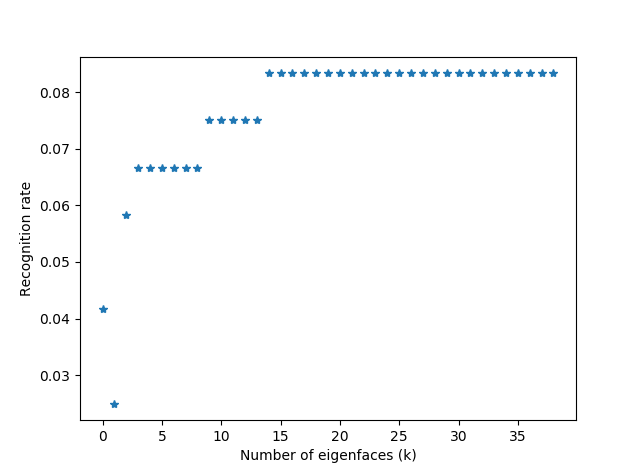
\includegraphics[scale=0.5]{img/tests/lwf/40ppl/PCA.png}
\caption{Recognition rate with varying number of eigenvectors for 20 individuals}
\end{figure} 

The question is how much can we improve our results with applying MLP network.


Model was trained with with following parameters:

\begin{itemize}
\itemsep0em
\item number of hidden layers = 1
\item initial weights chosen randomly in a range [0:1]
\item sigmoid activation function
\item learning parameter = 0.2
\end{itemize}

and various dimension of input data (amount of eigenfaces) and different amount of neurons in a hidden layer.

The training results are presented on figure (???):

\begin{figure}[H]
\centering
\begin{subfigure}[b]{.45\linewidth}
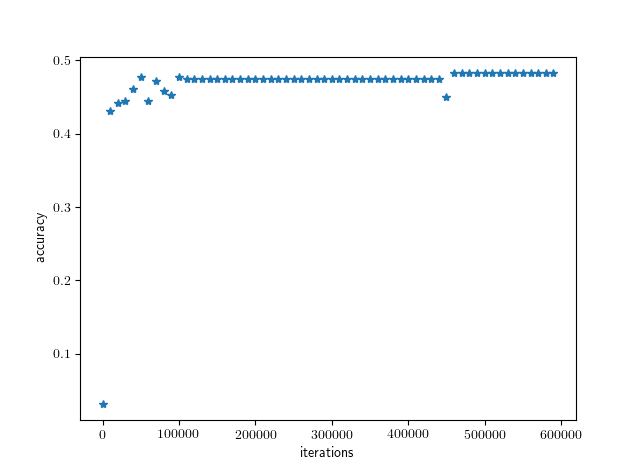
\includegraphics[width=\linewidth]{img/tests/lwf/40ppl/PCA_MLPk20h11}
\caption{10 hidden neurons, k = 15}
\end{subfigure}
\begin{subfigure}[b]{.45\linewidth}
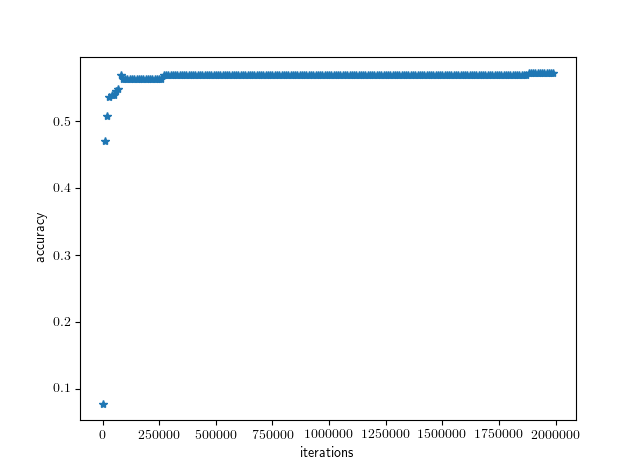
\includegraphics[width=\linewidth]{img/tests/lwf/40ppl/PCA_MLPk1520}
\caption{20 hidden neurons, k = 15}
\end{subfigure}


\begin{subfigure}[b]{.45\linewidth}
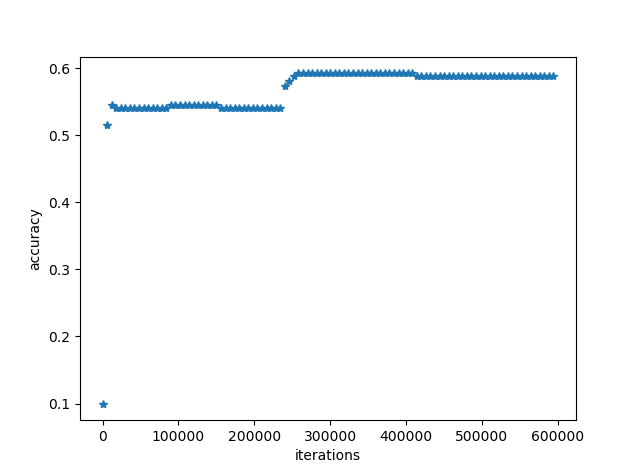
\includegraphics[width=\linewidth]{img/tests/lwf/40ppl/PCA_MLPk10h20}
\caption{10 hidden neurons, k = 10}
\end{subfigure}
\begin{subfigure}[b]{.45\linewidth}
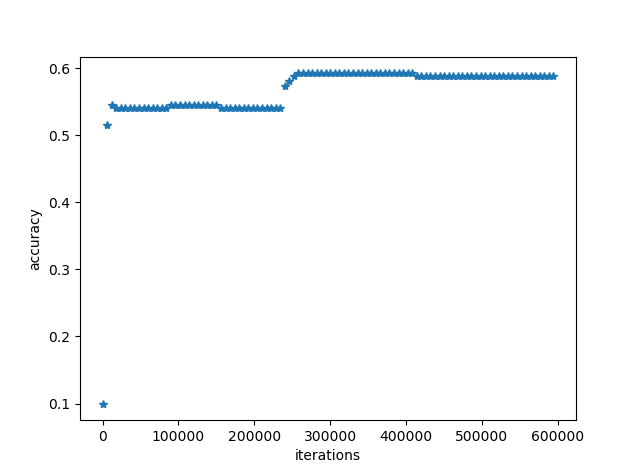
\includegraphics[width=\linewidth]{img/tests/lwf/40ppl/PCA_MLPk10h20.png}
\caption{20 hidden neurons, k = 10}
\end{subfigure}
\caption{Training accuracy for different amount of hidden neurons and eigenfaces}
\end{figure}

During experiment it was noticeable that the training accuracy grows with increasing the amount of hidden neurons. However, the time to train the network also grows and sometimes it was too long to see the performance:

\begin{figure}[H]
\centering
\begin{subfigure}[b]{.45\linewidth}
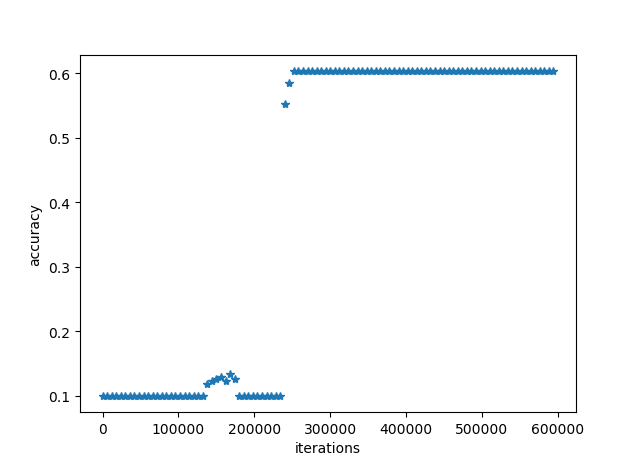
\includegraphics[width=\linewidth]{img/tests/lwf/40ppl/PCA_MLPk15h25}
\caption{25 hidden neurons, k = 15}
\end{subfigure}
\begin{subfigure}[b]{.45\linewidth}
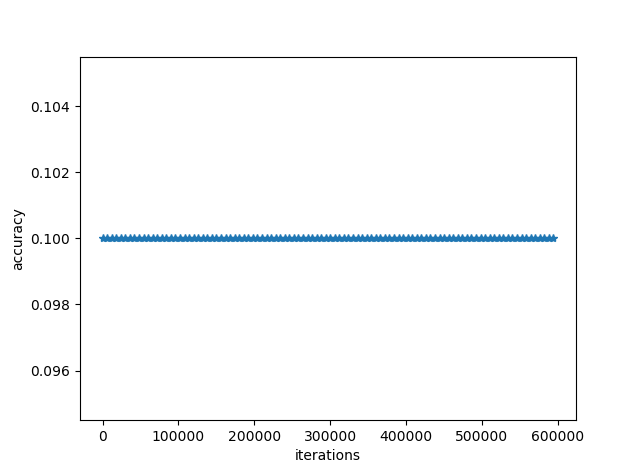
\includegraphics[width=\linewidth]{img/tests/lwf/40ppl/PCA_MLPk15h35.png}
\caption{30 hidden neurons, k = 15}
\end{subfigure}
\caption{Training accuracy for different amount of hidden neurons}
\end{figure}


After several experiments the best result was achieved with the model trained with 13 eigenfaces and 20 hidden neurons.


\begin{figure}[H]
\centering
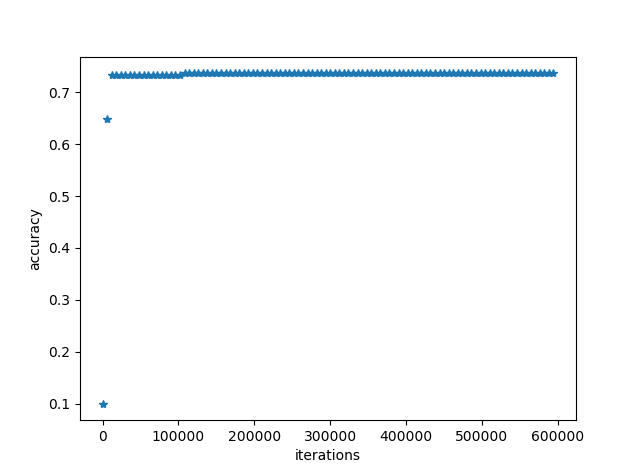
\includegraphics[scale=0.5]{img/tests/lwf/40ppl/PCAk15h20.png}
\caption{20 hidden neurons, k = 13}
\end{figure} 

The obtained recognition rate was 56.6\%, which is much better then PCA result but still not acceptable for facial recognition system. However, taking into consideration the quality and variety of images used for these tests, the result is better than expected.


\subsection{Two hidden layers}

Further experiments were performed on network topology presented on figure( ???). The goal is to check if additional hidden layer improves the network performance.

\begin{figure}[!h]
\centering
\begin{tikzpicture}[
           > = Stealth, semithick,
plain/.style = {draw=none, fill=none, yshift=11mm,
                text width=7ex,  align=center},% for text in images, 
   ec/.style = {draw=none},% for emty cells
  net/.style = {% for matrix style
    matrix of nodes,
    nodes={circle, draw, semithick, minimum size=12mm, inner sep=0mm},% circles in image
    nodes in empty cells,% for not used cells in matrix
  column sep = 16mm, % distance between columns in matrix 
     row sep = -3mm  % distance between rows in matrix
            },
]
\matrix[net] (m)% m is matrix name, it is used for names of cell: firs has name m-1-1
                % in empty space between ampersands will show circles: 
                % i.e.: nodes of the neural network
{
|[plain]| $Input$ & |[plain]| $Hidden_1$ &  |[plain]| $Hidden_2$& |[plain]| $Output$ \\
|[ec]|                &                         &                           & |[ec]|                  \\
                      & |[ec]|                  & |[ec]|                    & |[ec]|                  \\
|[ec]|                &                         &                           &                         \\
                      & |[ec]|                  & |[ec]|                   &  |[ec]|                  \\
|[ec]|                &                         &                           &                         \\
                      & |[ec]|                  & |[ec]|                    & |[ec]|                  \\
|[ec]|                &                         &                           & |[ec]|                  \\
};
\% inputs
\foreach \in [count=\ir from 1] in {3,5,7}
\draw[<-] (m-\in-1.west) -- node[above] {} +(-12mm,0);
% connections between nodes in the first and second layer
\foreach \j in {3,5,7}
{
\foreach \k in {2,4,6,8} \draw[->] (m-\j-1) -- (m-\k-2);
}
% connections between nodes in the second and third layer
\foreach \j in {2,4,6,8}
{
\foreach \k in {2,4,6, 8} \draw[->] (m-\j-2) -- (m-\k-3);
}

\foreach \j in {2,4,6,8}
{
\foreach \k in {4,6} \draw[->] (m-\j-3) -- (m-\k-4);
}
% output
% output
\draw[->] (m-4-4.east) -- node[above] {} +(12mm,0);
\draw[->] (m-6-4.east) -- node[above] {} +(12mm,0);
\end{tikzpicture}
\caption{Neural Network with two hidden layers}
\end{figure}

The first tests were ran with following parameters:

\begin{itemize}
\itemsep0em
\item number of hidden layers = 2
\item initial weights chosen randomly in a range [0:1]
\item sigmoid activation function
\item learning parameter = 0.2
\item number of eigenfaces = 15
\end{itemize}

Results are presented on figure( ??)


\begin{figure}[H]
\centering
\begin{subfigure}[b]{.45\linewidth}
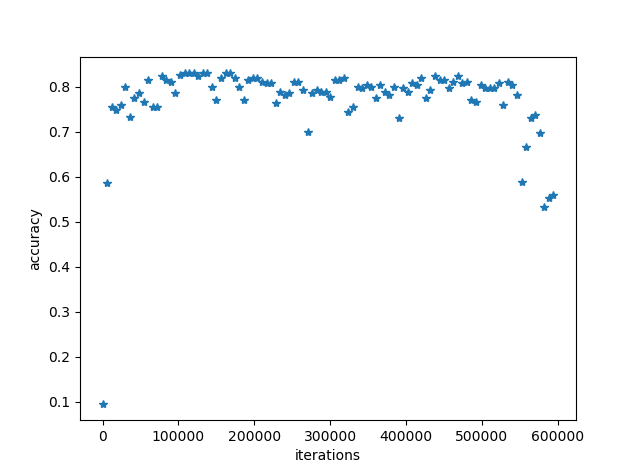
\includegraphics[width=\linewidth]{img/tests/lwf/40ppl/h2/PCA_MLP15_10_102.png}
\end{subfigure}
\begin{subfigure}[b]{.45\linewidth}
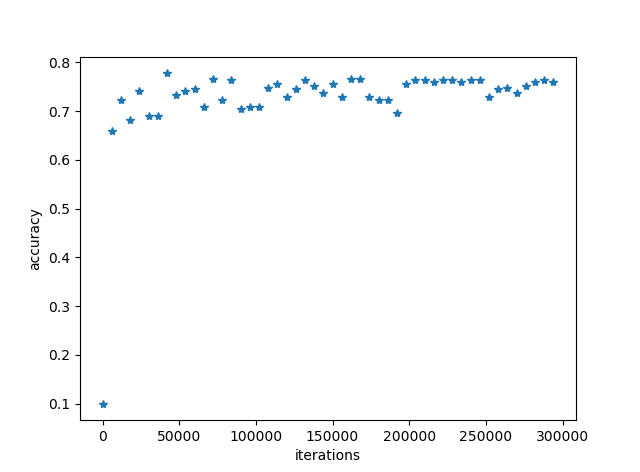
\includegraphics[width=\linewidth]{img/tests/lwf/40ppl/h2/PCA_MLP15_10_103.png}
\end{subfigure}
\caption{10 hidden neurons in each hidden layers, learning rate = 0.2}
\end{figure}

The system seemed to be very unstable. The learning rate was reduced to $0.05$ with the following results:

\begin{figure}[H]
\centering
\begin{subfigure}[b]{.45\linewidth}
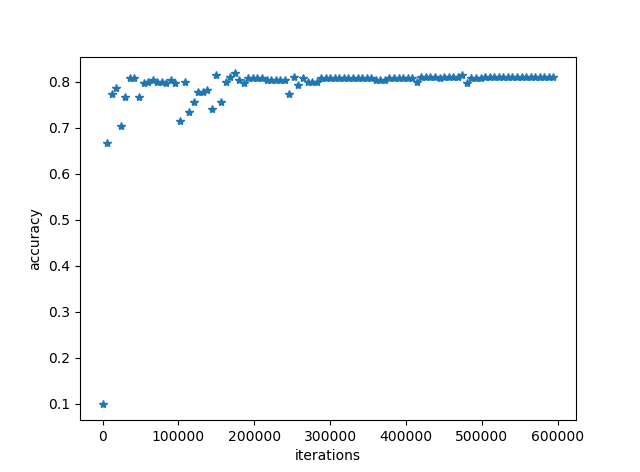
\includegraphics[width=\linewidth]{img/tests/lwf/40ppl/h2/PCA_MLP15_10_10.png}
\end{subfigure}
\begin{subfigure}[b]{.45\linewidth}
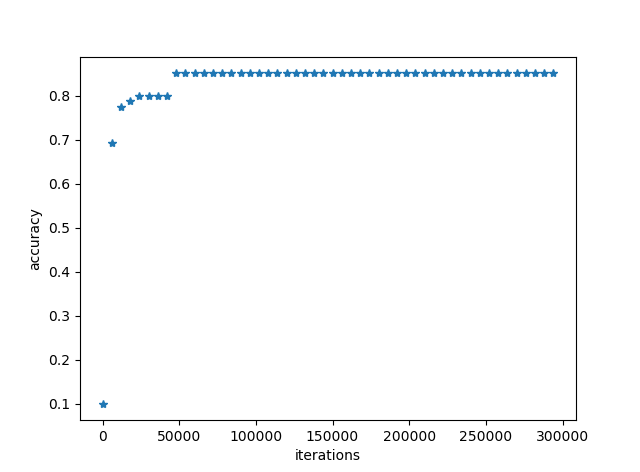
\includegraphics[width=\linewidth]{img/tests/lwf/40ppl/h2/PCA_MLP15_10_101.png}
\end{subfigure}
\caption{10 hidden neurons in each hidden layers, learning rate = 0.05}
\end{figure}


Better results were obtained with slightly bigger number of neurons in the second hidden layer. 

The network with following parameters gave the best training results:

\begin{itemize}
\itemsep0em
\item number of hidden layers = 2
\item 10 neurons in first hidden layer
\item 15 neurons in second hidden layer
\item initial weights chosen randomly in a range [0:1]
\item sigmoid activation function
\item learning parameter = 0.05
\item number of eigenfaces = 15
\end{itemize}


\begin{figure}[H]
\centering
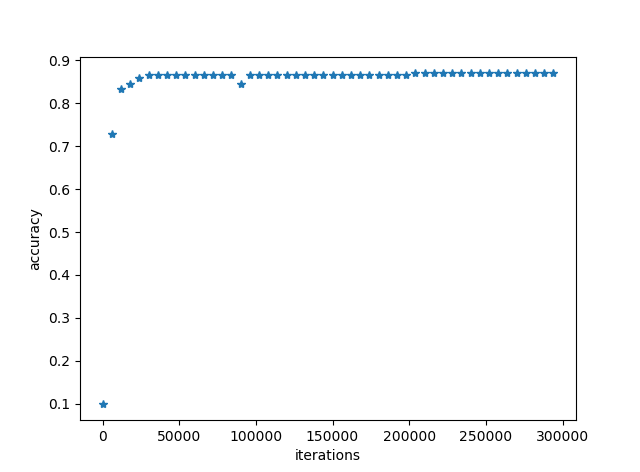
\includegraphics[scale=0.5]{img/tests/lwf/40ppl/h2/PCA_MLP15_10_104_best.png}
\caption{10 neurons in first hidden layer, 15 in the second hidden layer}
\end{figure}


The obtained recognition rate is 73.3\%. 

The presented results varies significantly on the values of initial weights and since the weights were chosen randomly it was a matter of error and trial to find an appropriate network configuration and train the network properly. It is possible that this score still can be improved. 


